%! Author = bedlamzd
%! Date = 28.02.2021

% Preamble
\documentclass[14pt]{extarticle}

%! Author = bedlamzd
%! Date = 16.02.2021

\usepackage{fontspec}
\usepackage{polyglossia}
\defaultfontfeatures{Ligatures=TeX}
\setdefaultlanguage{russian}
\setotherlanguage{english}
\setmainfont{PT Astra Serif}
\newfontfamily{\latinfont}{PT Astra Serif}
\newfontfamily{\cyrillicfont}{PT Astra Serif}
\newfontfamily{\cyrillicfonttt}{FreeMono}

\usepackage{geometry}

\usepackage{amsmath}
\usepackage{amssymb}
\usepackage{amsfonts}
\usepackage{graphicx}
\usepackage{float}
\usepackage{wrapfig}
\usepackage[caption=false]{subfig}

\geometry{right=20mm}
\geometry{left=20mm}
\geometry{top=20mm}
\geometry{bottom=20mm}

\usepackage{indentfirst}
\usepackage[outputdir=out]{minted}

\renewcommand{\theFancyVerbLine}{\ttfamily{\normalsize\oldstylenums{\arabic{FancyVerbLine}}}}

\newminted{python}{autogobble, linenos, fontsize=\small, xleftmargin=2\parindent}
\newmintinline{python}{fontsize=\small}
\newmintedfile{python}{autogobble, linenos, fontsize=\small, xleftmargin=2\parindent,
breakanywhere, breaklines}

\newminted{matlab}{autogobble, linenos, fontsize=\small, xleftmargin=2\parindent}
\newmintinline{matlab}{fontsize=\small}
\newmintedfile{matlab}{autogobble, linenos, fontsize=\small, xleftmargin=2\parindent,
breakanywhere, breaklines}

\renewcommand{\thesubsection}{\arabic{subsection}}

\graphicspath{{../img/}}



% Document
\begin{document}
    \begin{titlepage}
    \begin{center}
        \begin{small}
            \textbf{Министерство науки и высшего образования Российской Федерации}

            \vspace{1em}

            ФЕДЕРАЛЬНОЕ ГОСУДАРСТВЕННОЕ АВТОНОМНОЕ ОБРАЗОВАТЕЛЬНОЕ\\
            УЧРЕЖДЕНИЕ ВЫСШЕГО ОБРАЗОВАНИЯ

            \vspace{1em}

            \textbf{<<НАЦИОНАЛЬНЫЙ ИССЛЕДОВАТЕЛЬСКИЙ УНИВЕРСИТЕТ ИТМО>>}
        \end{small}

        \vspace{13ex}

        Практическая работа №4\\
        <<Планирование движения>>\\
        по дисциплине <<Моделирование и управление робототехническими системами>>
    \end{center}

    \vspace{14em}

    \begin{flushright}
        \noindent
        Выполнил:\\
        студент гр. R41341c\\
        Борисов М. В.

        \vspace{1em}
        Преподаватель:\\
        Каканов М. А.
    \end{flushright}

    \vfill

    \begin{center}
        \large{Санкт-Петербург}\\
        2021 г.\\
    \end{center}
\end{titlepage}


    \section*{Дано}
    Модель двухзвенного робота
    \begin{equation}
        \label{eq:sys}
        M(q)\ddot{q} + C(q, \dot{q})\dot{q} + F\dot{q} +G(q) = u,
    \end{equation}
    где $q,\ \dot{q},\ \ddot{q}$ --- векторы обобщённых координат, скоростей и ускорений соответственно,
    $u$ --- вектор управляющих воздействий,
    $M(q),\ C(q,\dot{q}),\ F$ --- матрицы инерции, кориолисовых-центробежных сил и вязкого трения соответственно,
    $G(q)$ --- вектор гравитационных сил.
    \newline

    Задающий сигнал
    \begin{equation}
        \label{eq:traject}
        q_{\text{ref}}(t) =
        \begin{bmatrix}
            A_{\text{ref},\ 1}\sin(\omega_{\text{ref},\ 1}t + \psi_{\text{ref},\ 1})\\
            A_{\text{ref},\ 2}\sin(\omega_{\text{ref},\ 2}t + \psi_{\text{ref},\ 2})
        \end{bmatrix}
    \end{equation}

    Цель управления
    \begin{equation}
        \label{eq:goal}
        \lim_{t \rightarrow \inf }\left| q_e(t) \right| = 0,
    \end{equation}
    где $q_e(t) = q(t) - q_\text{ref}(t)$ --- сигнал ошибки.

    \section*{Задание}
    \paragraph*{Задание 1} Управление роботом по состоянию

    \subparagraph{Допущение 1} Вектор обобщённых скоростей $\dot{q}(t)$ доступен измерению.

    \subparagraph{Допущение 2} Матрицы $M(q),\ C(q, \dot{q}),\ F,\ G(q)$ известны. \\

    \noindent Закон управления
    \begin{equation}
        \label{eq:control by speed}
        u = M(q)\left( \ddot{q_\text{ref}} - K_p q_e - K_d\dot{q_e}) \right) + C(q, \dot{q})\dot{q} + F\dot{q} + G(q),
    \end{equation}
    где $K_p$ и $K_d$ --- соответственно матрицы пропорциональных и дифференциальных коэффициентов.
    \newline

    Требуется провести численное моделирование замкнутой системы~\eqref{eq:sys},~\eqref{eq:control by speed}
    в режиме слежения за траекторией~\eqref{eq:traject} с обеспечением цели управления~\eqref{eq:goal}.

    \paragraph*{Задание 2} Управление роботом по выходу

    Ослабим Допущение 1 и построим регулятор по выходу. Выберем закон управления
    \begin{equation}
        \label{eq:control no speed}
        u = M(q)\left( \ddot{q_\text{ref}} - K_p q_e - K_d \left( \hat{\dot{q}} - \dot{q_\text{ref}} \right)) \right) + C(q, \hat{\dot{q}})\hat{\dot{q}} + F\hat{\dot{q}} + G(q),
    \end{equation} где $K_p$ и $K_d$ --- соответственно матрицы пропорциональных и дифференциальных коэффициентов,
    $\hat{\dot{q}}$ --- оценка обобщённой скорости, полученная с помощью фильтра на базе расширенного наблюдателя.

    Требуется провести численное моделирование замкнутой системы~\eqref{eq:sys},~\eqref{eq:control no speed}
    в режиме слежения за траекторией~\eqref{eq:traject} с обеспечением цели управления~\eqref{eq:goal}.

    \section*{Моделирование}
    \subsection*{Задание 1}
    В пакете MATLAB соберём систему~\eqref{eq:sys},~\eqref{eq:control by speed} в виде модели Simulink.
    \begin{figure}[H]
        \centering
        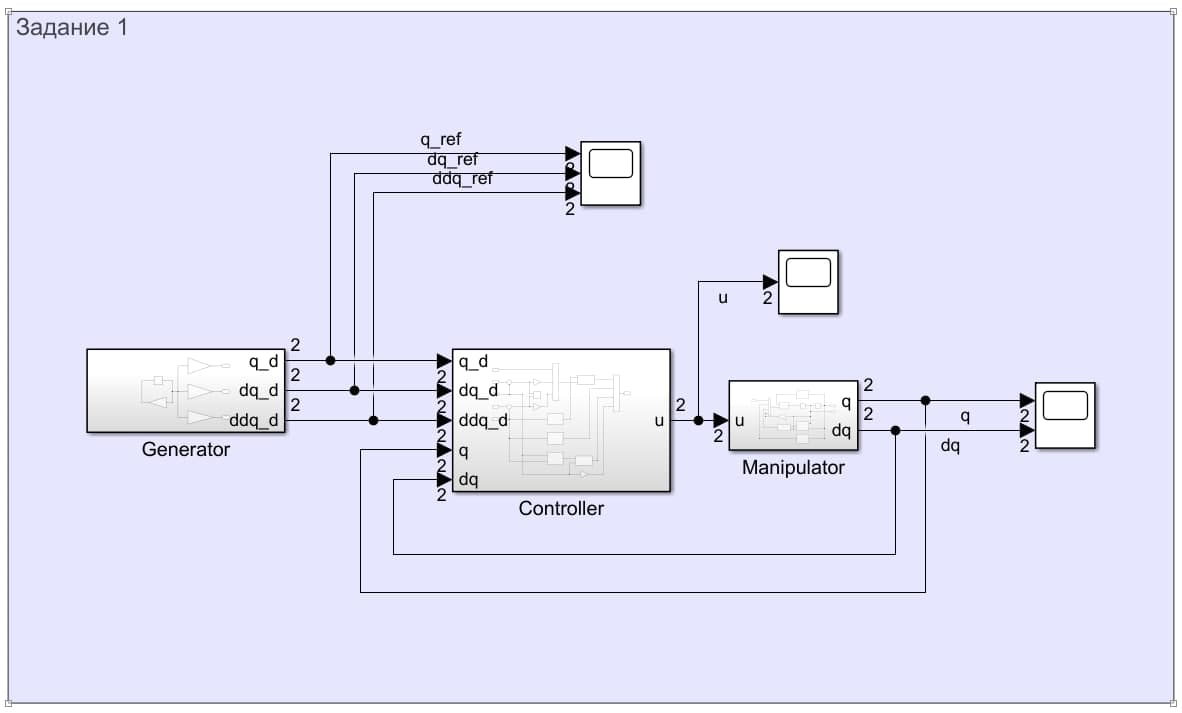
\includegraphics[width=0.75\textwidth]{global sys.jpg}
        \caption{Общий вид модели в MATLAB}
        \label{pic:global sys}
    \end{figure}

    Инициализация всех параметров производится с помощью автоматически вызываемой встроенной функции \texttt{InitFcn},
    где перечисленны необходимые переменные (см.~\ref{code:given}).
    \begin{figure}[H]
        \centering
        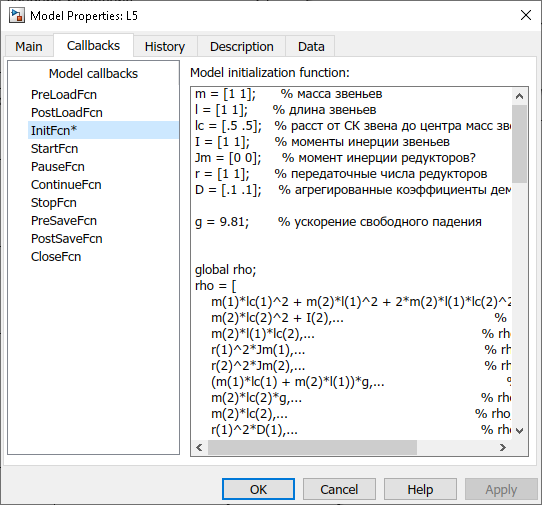
\includegraphics[height=0.3\textheight]{InitFcn.png}
        \caption{Окно \texttt{InitFcn}}
        \label{pic:InitFcn}
    \end{figure}

    \sloppy Модель манипулятора представлена на рисунке~\ref{pic:manipulator}, где матрицы $M(q),\ C(q, \dot{q}),\ G(q)$ представлены блоками
    \texttt{MATLAB Function}. (см.~\ref{code:matricies})
    \begin{figure}[H]
        \centering
        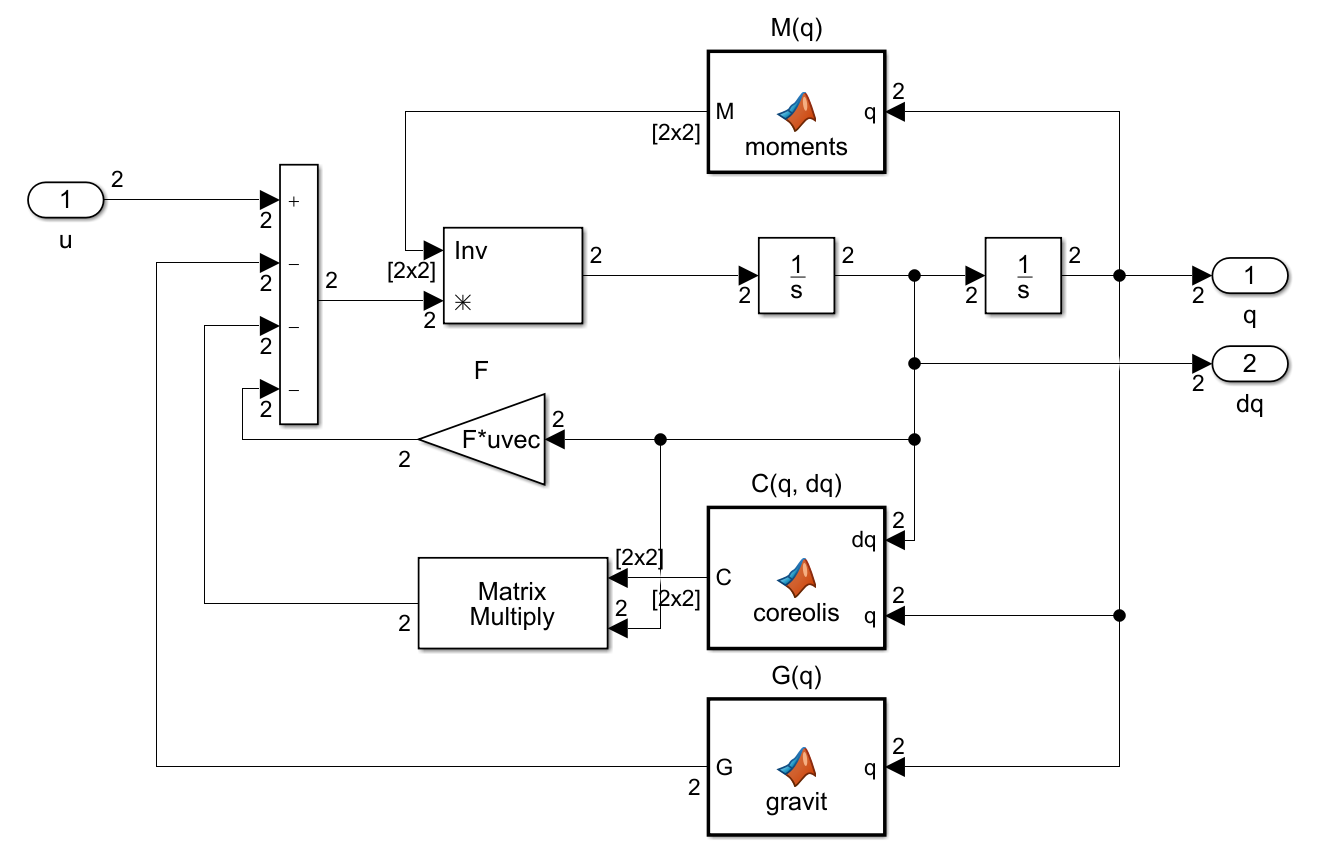
\includegraphics[width=0.75\textwidth]{manipulator.png}
        \caption{Модель манипулятора}
        \label{pic:manipulator}
    \end{figure}

    Модель регулятора представлена на рисунке~\ref{pic:controller no observer}, при этом по допущению 2 мы можем использовать
    матрицы напрямую, которые представлены уже показанными блоками функций.
    \begin{figure}[H]
        \centering
        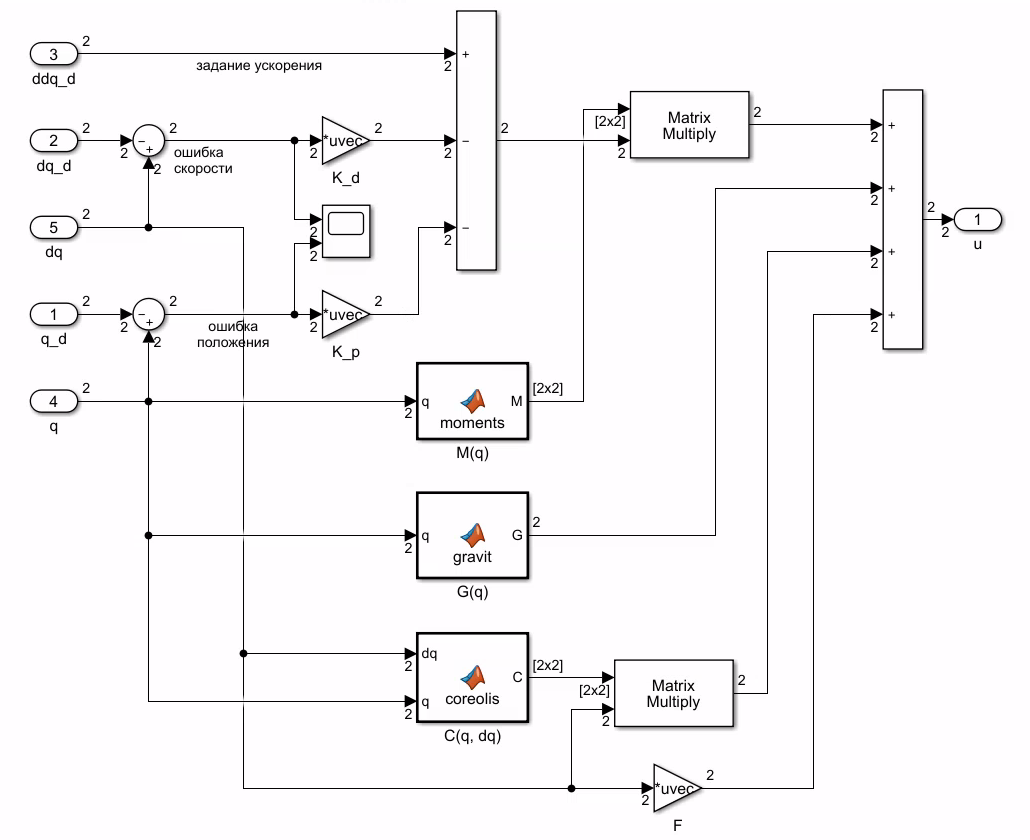
\includegraphics[width=0.75\textwidth]{controller no observer.png}
        \caption{Модель регулятора}
        \label{pic:controller no observer}
    \end{figure}

    Генератор задающего воздействия~\eqref{eq:traject} представлен на рисунке~\ref{pic:generator}
    \begin{figure}[H]
        \centering
        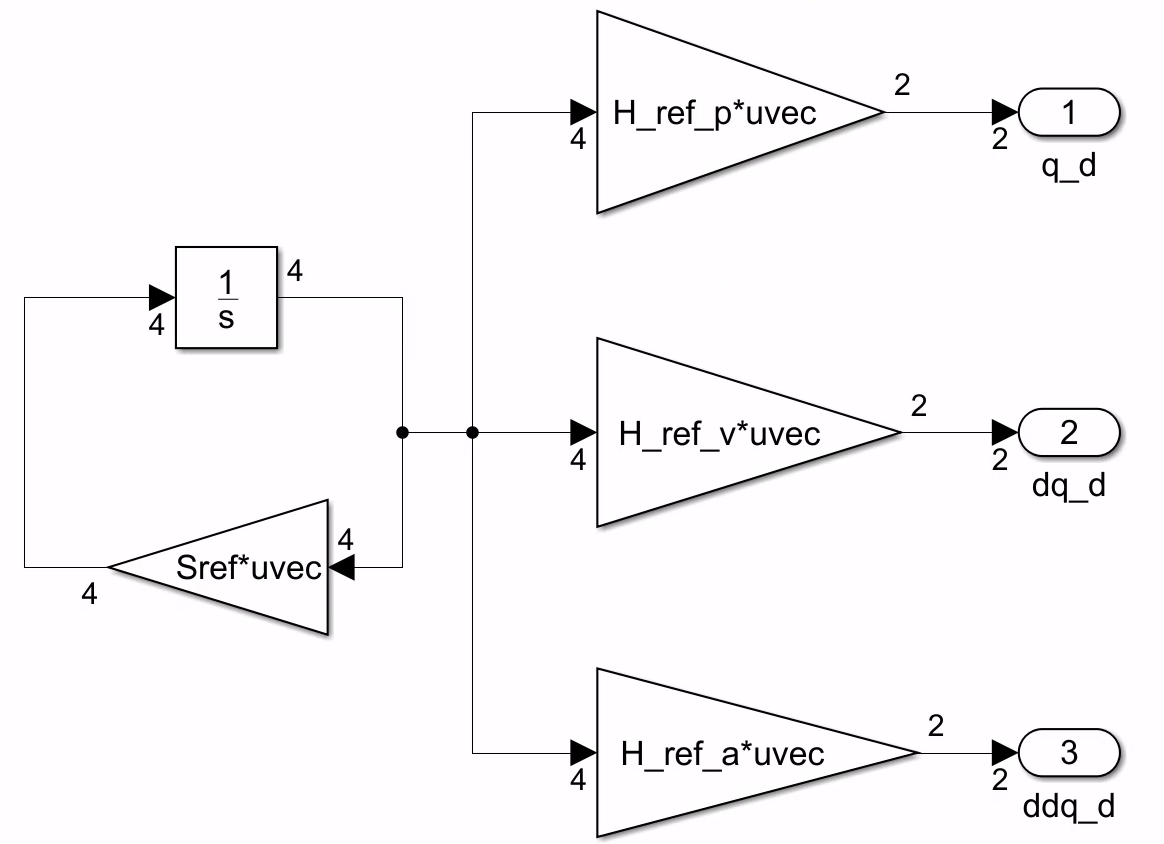
\includegraphics[width=0.75\textwidth]{generator.png}
        \caption{Модель задающего воздействия}
        \label{pic:generator}
    \end{figure}

    Результат моделирования представлен на рисунке~\ref{pic:result by speed}. По графику очевидно, что ошибка
    положения звеньев сходится к нулю и соответственно цель моделирования~\eqref{eq:goal} выполнена.
    \begin{figure}[H]
        \centering
        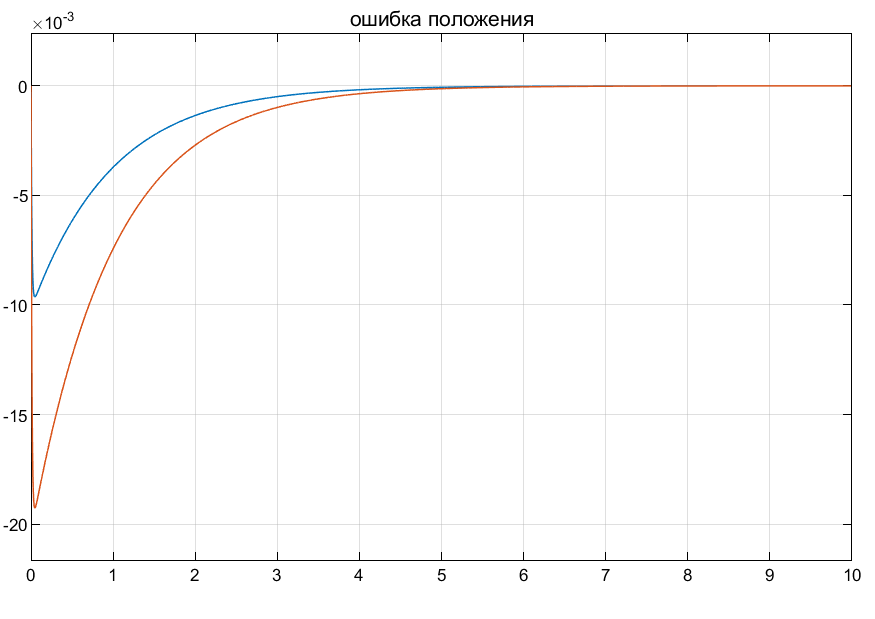
\includegraphics[width=0.75\textwidth]{result by speed.png}
        \caption{Ошибка положения системы}
        \label{pic:result by speed}
    \end{figure}

    \subsection*{Задание 2}
    Ослабив допущение 1 мы более не имеем возможности напрямую измерять скорость звеньев манипулятора
    и модель изменяется соответственно.

    В блок регулятора (рисунок~\ref{pic:controller observer}) добавляется расширенный наблюдатель,
    представленный на рисунке~\ref{pic:extended observer}, задача которого давать оценку вектора
    обобщённой скорости.
    \begin{figure}[H]
        \centering
        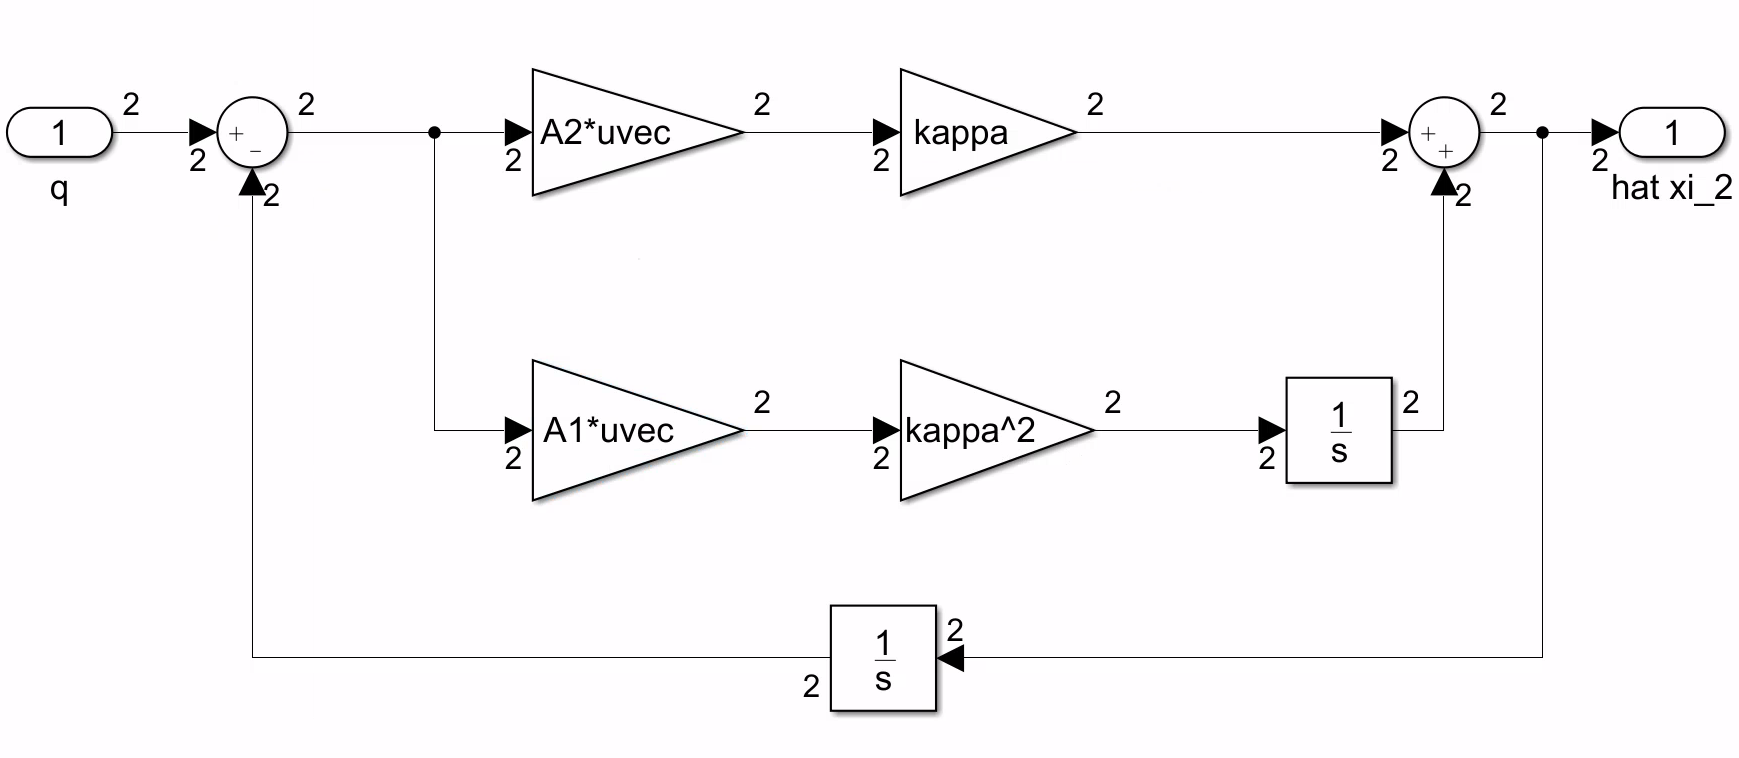
\includegraphics[height=0.2\textheight]{extended observer.png}
        \caption{Модель расширенного наблюдателя}
        \label{pic:extended observer}
    \end{figure}

    \begin{figure}[H]
        \centering
        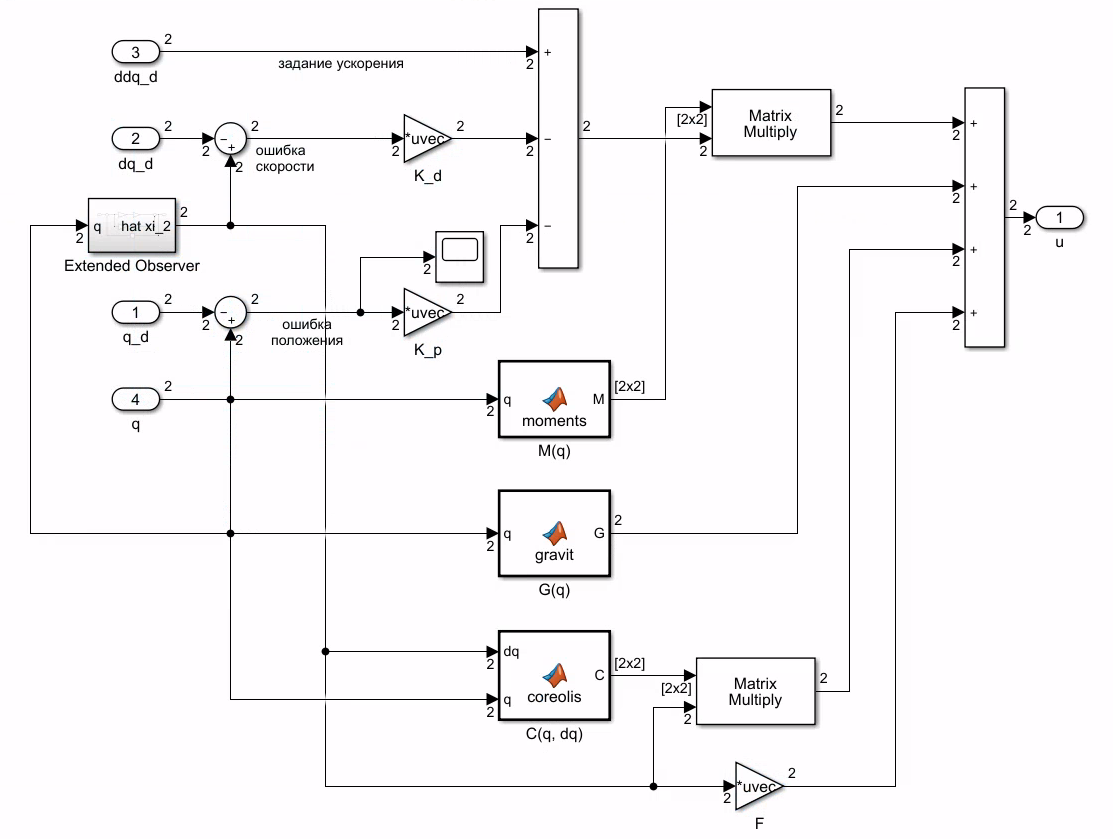
\includegraphics[width=0.75\textwidth]{controller observer.png}
        \caption{Модель регулятора с расширенным наблюдателем}
        \label{pic:controller observer}
    \end{figure}

    Результат моделирования представлен на рисунке~\ref{pic:result no speed}. По графику очевидно, что ошибка
    положения звеньев сходится к нулю и соответственно цель моделирования~\eqref{eq:goal} выполнена.
    \begin{figure}[H]
        \centering
        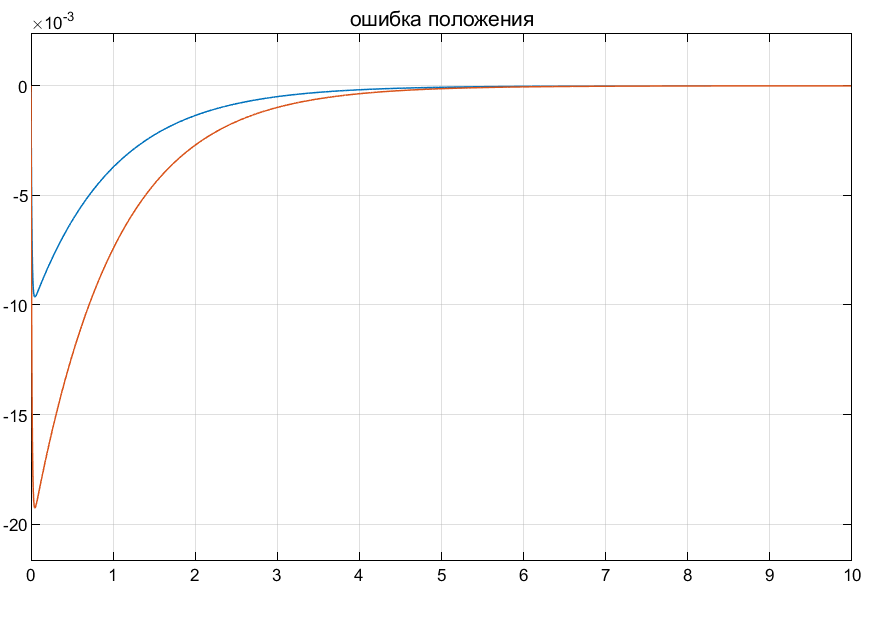
\includegraphics[width=0.75\textwidth]{result no speed.png}
        \caption{Ошибка положения системы}
        \label{pic:result no speed}
    \end{figure}

    \section*{Вывод}
    В работе было промоделировано управление двухзвенным манипулятором с помощью ПД-регулятора.
    Результаты моделирования показывают, что использование расширенного наблюдателя в системе без
    обратной связи по скорости позволяет успешно управлять объектом и ошибка положения сходится
    к нулю так же как и при возможности измерения скорости.

    \appendix \newpage
    \renewcommand{\thesection}{Приложение \Asbuk{section}}
    \section{Параметры инициализации}\label{code:given}
    \octavefile[frame=single]{../src/given.m}

    \newpage
    \section{Блоки расчёта матриц}\label{code:matricies}
    \begin{octavecode*}{frame=single}
        function M = moments(q)
            global rho;
            c2 = cos(q(2));
            M = [
                rho(1) + rho(2) + 2*rho(3)*c2 + rho(4) rho(2) + rho(3)*c2;
                rho(2) + rho(3)*c2 rho(2) + rho(5);
                ];
        end

        function C = coreolis(dq, q)
            global rho;
            s2 = sin(q(2));
            C = [
                -rho(3)*s2*dq(2) -rho(3)*s2*(dq(1) + dq(2));
                rho(3)*s2*dq(1) 0
                ];
        end

        function G = gravit(q)
            global rho;
            c1 = cos(q(1));
            c12 = cos(q(1) + q(2));
            G = [
                rho(6)*c1 + rho(7)*c12;
                rho(8)*c12
                ];
        end
    \end{octavecode*}


\end{document}
